
\documentclass[aps, prd, superscriptaddress,twocolumn,amsmath,amssymb,nofootinbib]{revtex4-1}
%\documentclass[prl,superscriptaddress,amsmath]{revtex4-1}
\usepackage{graphicx}
%\usepackage{float}
\usepackage{color}
%\usepackage{tensor}
\usepackage{epstopdf,cancel,ulem}
\usepackage{epsf,latexsym,bbm,euscript}
\usepackage{amssymb,amsmath}
\usepackage{mathtools} %used in this file for the command \coloneqq -> :=
\usepackage{times,graphics}
%\usepackage{subfig}
\usepackage{soul,xcolor}
\usepackage{epsfig}
%\usepackage{geometry}

\linespread{1.0}
% \usepackage{geometry}
\usepackage{graphicx}
%\usepackage{maplestd2e}
%\usepackage[dvipsnames]{xcolor}
%\usepackage{epstopdf}
%\usepackage[abs]{overpic}
%\usepackage{color}
%\usepackage{comment}
%\usepackage{float}
% \usepackage{showkeys}
%\usepackage{booktabs}
\usepackage[colorlinks]{hyperref}


%%%%%%%%%%%%%%%%%%%%%%%%%%%%%%%%%%%%%%%%%%%%%%%%%%%%%%
%% definitions
\newcommand{\ph}{\varphi}
\newcommand{\tht}{\vartheta}
\newcommand{\eps}{\varepsilon}
\newcommand{\one}{\textsc{i}}

 \newcommand{\dm}{n}

\newcommand{\tens}[1]{{\boldsymbol{#1}}} 
\newcommand{\pa}{{\tens{\partial}}}

\newcommand{\be}{\begin{equation}}
\newcommand{\ee}{\end{equation}}
\newcommand{\ba}{\begin{eqnarray}}
\newcommand{\ea}{\end{eqnarray}}

\newcommand{\beq}{\begin{equation}}
\newcommand{\eeq}{\end{equation}}
\newcommand{\beqa}{\begin{eqnarray}}
\newcommand{\eeqa}{\end{eqnarray}}
\newcommand{\nn}{\nonumber}
\newcommand{\tcb}{\textcolor{blue}}
\newcommand{\tcr}{\textcolor{red}}


\newcommand{\hook}{\raisebox{-0.35ex}{\makebox[0.6em][r]
{\scriptsize $-$}}\hspace{-0.15em}\raisebox{0.25ex}{\makebox[0.4em][l]{\tiny
 $|$}}}
\newcommand{\cwedge}[1]{\mathop{\wedge}_{{}^{#1}} }

\newcommand{\even}{{\mathrm{e}}}
\newcommand{\odd}{{\mathrm{o}}}
\newcommand{\KY}{{\scriptscriptstyle\mathrm{KY}}}
\newcommand{\SN}{{\scriptscriptstyle\mathrm{SN}}}

\newcommand{\fiber}{\boldsymbol}

\newcommand{\lied}{\mathcal{L}}
%\newcommand{\cd}[1]{\frac{\partial}{\partial{#1}}}
\newcommand{\cd}[1]{\frac{\eth}{\partial{#1}}}
\newcommand{\cv}[1]{{\partial}_{#1}}

\newcommand{\Ric}{{\mathrm{Ric}}}
\newcommand{\curvop}{{\boldsymbol{\mathsf{R}}}}
\newcommand{\sccur}{{\mathcal{R}}}
\newcommand{\detg}{{\mathfrak{g}}}


\newcommand{\gc}[2]{{[\mspace{-4mu}\lvert#1,#2\rvert\mspace{-4mu}]}}
\newcommand{\bgc}[2]{{\bigl[\mspace{-4.4mu}\lvert#1,#2\rvert\mspace{-4.4mu}\bigr]}}
\newcommand{\Bgc}[2]{{\biggl[\mspace{-5mu}\Bigl\lvert#1,#2\Bigr\rvert\mspace{-5mu}\biggr]}}

\newcommand{\lst}[1]{\langle{#1}\rangle}


\newcommand{\ef}{E}
\newcommand{\efr}{{\underset{\raisebox{0.5ex}{$\scriptscriptstyle\rightarrow$}}{e}\mspace{-2mu}}}
\newcommand{\Xfr}{{\overset{\raisebox{-0.5ex}{$\scriptscriptstyle\rightarrow$}}{X}\mspace{-1mu}}}



\newcommand{\spcm}{{\mspace{14.5mu}}}                  % space with width of minus
\newcommand{\nquad}{{\mspace{-20mu}}}                  % negative quad
\newcommand{\textdash}{{\text{-}}}                     % text dash for equations



\newcommand{\KV}[1]{\xi_{(#1)}}
\newcommand{\KT}[1]{K_{(#1)}}
\newcommand{\PKV}{\xi}
\newcommand{\CCKY}[1]{h^{(#1)}}


\newcommand{\A}[1]{A^{\!(#1)}}
\newcommand{\B}[1]{B^{\!(#1)}}
\newcommand{\Bo}[1]{\mathcal{B}^{(#1)}}
\newcommand{\Vo}{\mathcal{V}}
\newcommand{\C}[1]{{\cal{#1}}}
\newcommand{\psc}[1]{\Psi_{#1}}
\newcommand{\chc}[1]{\mathcal{X}_{#1}}
\newcommand{\psf}[1]{\tilde\Psi_{#1}}
\newcommand{\chf}[1]{\tilde{\mathcal{X}}_{#1}}

\newcommand{\clfm}[1]{{\slash\mspace{-9.5mu}{#1}}}
\newcommand{\Ha}{{\cal{H}}}


\def\Gdp{\Gamma_{\mathrm{DP}}}
\def\Gktm{\Gamma_{\mathrm{KTM}}}
\def\tGktm{\tilde{\Gamma}_{\mathrm{KTM}}}

%\newcommand{\comment}[2][]{\noindent\hspace{-4em}\framebox{\parbox{6.5in}{\textsf{\small\emph{Comment by #1:} #2}}}\medskip}

%\input{tex_defs}

%%%%%%%%%%%%%%%%%%%%%%%%%%%%%%%%%
%%% definitions of common symbols %%%%%%%
% two particle density operator \
\def\Rt{{\rho}_{12}(t)}
% one particle density operator 
\def\rt{{\rho}(t)}
\def\drho{\dot\rho}
% bra and  kets
\newcommand{\ket}[1]{\lvert \, #1\rangle}
\newcommand{\bra}[1]{\langle #1 \, \rvert}
\newcommand{\braket}[2]{\langle #1 \, | \, #2 \rangle}
\newcommand{\mean}[1]{\langle #1 \rangle}
% "hats"
\newcommand{\h}[1]{\hat#1{}}
%trace 
\def\Tr{{\textrm{Tr}}}


\newcommand{\Radd}[1]{\textcolor{blue}{#1} }
\newcommand{\Rcomm}[1]{\textcolor{blue}{\bf{[#1]}} }
\newcommand{\Nadd}[1]{\textcolor{violet}{#1} }
\newcommand{\Ncomm}[1]{\textcolor{violet}{\bf{[#1]}} }
\newcommand{\f}{\textcolor{cyan}}
\newcommand{\green}{\textcolor{green}}
\newcommand{\mz}[1]{\textcolor{cyan}{#1} }
\newcommand{\mzc}[1]{\textcolor{cyan}{\bf{[#1]}} }
\newcommand{\red}[1]{\textcolor{red}{#1}}

\begin{document}
\begin{titlepage}
    \begin{center}
        \vspace*{3cm}
        
       \textbf{\huge Gravity May Be a Pairwise Local Classical Channel}
               
        \vspace{1.5cm}
        \textbf{Jamie Breault}
        
        \today
        
        \vspace{1.5cm}
        A report presented as partial fulfilment of the\\
        requirements of Physics 437A 
        \vspace{3cm}
        \end{center}
        
        Many models have been proposed to describe gravity according to the principles of quantum mechanics. However, until direct experimental evidence of quantum gravity is found, gravity being fundamentally classical remains a valid possibility. Kafri, Taylor, and Milburn purpose a model where gravity is a pairwise local classical channel. Altamirano, Corona-Ugalde, Mann, and Zych compared this model to atomic fountain interference experiments using a maximum visibility estimate derived through decoherence rate minimization. Here I show that the atom's true theoretical maximum visibility must be derived using heating rate minimization instead. It is then shown that this model of classical gravity predicts maximum visibility values greater than the those measured experimentally. For this reason, gravity may be a pairwise local classical channel.
    
    \newpage
\end{titlepage}
\onecolumngrid
\pagenumbering{roman}
\tableofcontents
\makeatletter
\let\toc@pre\relax
\let\toc@post\relax
\makeatother
\newpage
\listoffigures
\newpage
\onecolumngrid
%\raggedright
\section{Introduction}
\pagenumbering{arabic}
Presently, one of the greatest problems in theoretical physics is unifying Einstein's theory of general relativity, which describes gravity, with quantum mechanics, which describes the other three fundamental forces. Many models have been proposed to describe gravity according to the principles of quantum mechanics, including loop quantum gravity and string theory \cite{PI}. However, there is not yet any direct observational evidence of quantum gravity \cite{no_QG_evidence}, thus gravity being fundamentally classical remains a valid possibility.

Measurement-feedback models of gravity purposed by Kafri, Taylor, and Milburn (KTM) \cite{KTM1, KTM2, KTM3} describe a mechanism by which gravity could be a classical channel, meaning that gravity would be unable to increase the entanglement of a system. Measurement-feedback models of gravity require agents to conduct measurements of particles' positions and then give corresponding feedback to other gravitationally interacting particles \cite{P6}. These agents are called ancillae \cite{P2}. Under the pairwise model of gravity, a system requires two ancillea for each pair particles present \cite{P3}.

Atomic fountain interference experiments \cite{kovachy, sugarbaker} can be used to test the legitimacy of pairwise gravity. To do so, the maximum visibility predicted by the model must be derived and compared to experiment. Visibility ranges from $0$ to $1$, and is a measure of the amount of a time a particle in a superposition can remain in a superposition. A particle with a visibility of $1$ will maintain its superposition size for all time, and a particle with a visibility of $0$ collapses to a single state immediately. There are two methods that can be used to estimate maximum visibility, one involves decoherence rate minimization and the other involves heating rate minimization \cite{P3}. The maximum visibility estimates produced by these methods may not be equal. The true theoretical maximum visibility is the greater of the two estimates. Altamirano, Corona-Ugalde, Mann, and Zych show in ref.~\cite{P3} that the maximum visibility estimate produced by minimizing decoherence rate does not agree with the atomic fountain experiments. Here I derive the estimate produced by minimizing heating rate instead, from which the true theoretical maximum visibility can be determined and compared to the values determined experimentally.

%%%%%%%%%%%%%%%%%%%%%%%%%%%%%%%%%%%%%%%%%%%%%%%%%%%%%

\section{Gravity as a Pairwise Classical Channel}

All fundamental forces are either a quantum channel or a classical channel (fig~\ref{Channels}), the difference being that quantum channels can increase the entanglement of a system and classical channels can not. Charged particles can interact through the quantum channel of electromagnetism. For example, consider an electron in a superposition, thus producing a quantum electrical potential. If another electron is introduced to this potential, it will be forced into a superposition as well due to the potential's quantum nature. The quantum potential entangles the two electrons. If an observation is made on either of the electrons, both electrons undergo decoherence due to their entanglement. Decoherence is the process of superposition size decreasing due to observation \cite{P6}.

Now consider a particle with mass in a superposition. If gravity is a classical channel, then another particle introduced to the gravitational potential of the first is not forced into a state of superposition. The second particle responds to the potential as though it is classical. It can be shown that a classical channel is equivalent to an agent performing weak measurements of the first particle's position and using the measurement outcomes to control the potential the other particle responds to. In other words, the second particle continually makes classical estimates of the potential. The pair of particles therefore never become entangled \cite{P6}. Note, if gravity is a classical channel, that does not imply that the entanglement of a gravitationally interacting system particles can not increase, it only implies that the entanglement can not increase due to gravity. The entanglement can still increase through quantum channels such as electromagnetism if the particles are charged, for example.

 \begin{figure*}[ht!]
 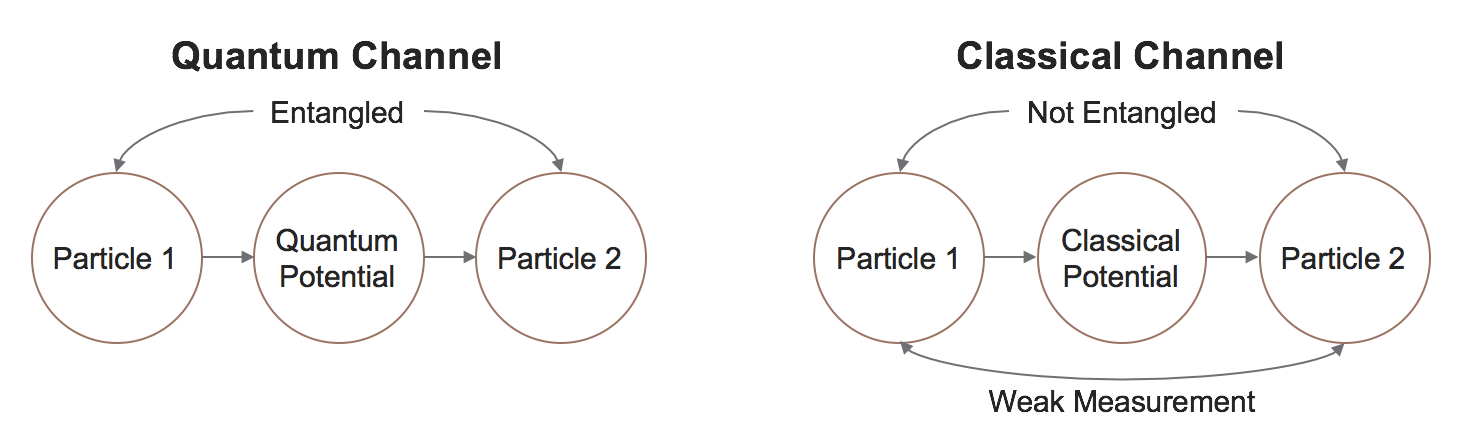
\includegraphics[width=0.8\textwidth]{Channel.png} 
\caption{Diagrams highlighting the differences between quantum channels (left) and classical channels (right).}
\label{Channels}
\end{figure*}

In the KTM model, the weak measurements are performed by force-carrying particles called ancillae. Gravity under this model can either be pairwise or global. In the pairwise case, a system requires two ancillae for every pair of gravitationally interacting particles. A system of two particles contains only a single pair, thus two ancillae are required. A system with three particles contains three pairs, thus six ancillae are required. The number of required ancillae increases rapidly as the number of particles increases. In the global case, only one ancilla is required for each particle in the system. Since the number of ancillae is always equal to number of particles in the global case, the global case predicts far fewer ancillae than the pariwise case for systems containing a large number of particles \cite{P3}. Here, only the pairwise case is considered due to time constraints. 

Ancillae propagate gravity through a measurement-feedback mechanism. To understand this mechanism, consider a simple system containing two particles and two ancillae (fig~\ref{measurement-feedback}). First, each ancilla interacts with a one of the two particles. These initial interactions are referred to as measurements because the ancillae are conducting weak measurments of the particles' positions. Each ancilla then interacts with the opposite particle, giving the particles feedback that depends on the outcome of the earlier measurement. The position of each particle shifts as a result of the feedback \cite{P2}.

 \begin{figure*}[ht!]
 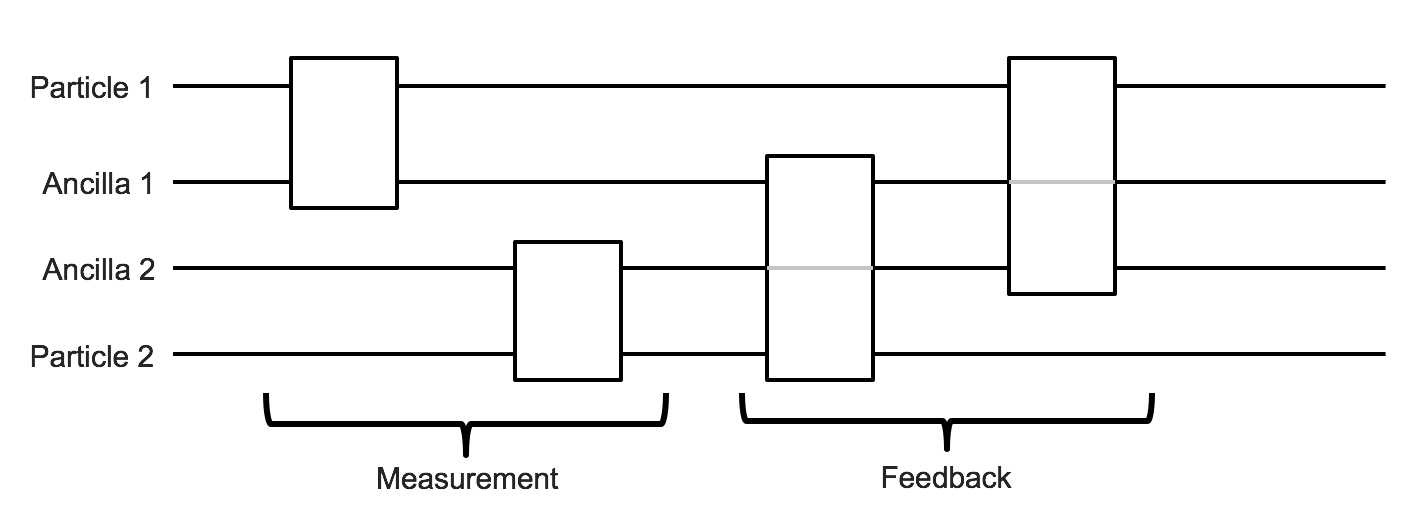
\includegraphics[width=0.8\textwidth]{Pairwise.png} 
\caption{Quantum circuit diagram illustrating the measurement-feedback mechanism by which ancillae propagate gravity.}
\label{measurement-feedback}
\end{figure*}

%%%%%%%%%%%%%%%%%%%%%%%%%%%%%%%%%%%%%%%%%%%%%%%%%%%%%

\section{Atomic Fountain Interference Experiments}

The atomic fountain interference experiments outlined in ref.~\cite{kovachy, sugarbaker} use large momentum transfer interferometers to put $^{87}$Rb atoms in a vertical spatial superposition. This is done using a sequence of $N$ $\frac{\pi}{2}$-pulses from a laser. The laser increases the superposition size for a total time $T$. The resulting superposition size of the atom is given by

\beq
\Delta x(t)=\frac{2\hbar N k  t}{m_a} 
 \label{SP_size}
 \eeq
 
 for $t<T$ where $k$ is the laser's wave-number and $m_a$ is the mass of a $^{87}$Rb atom.

%%%%%%%%%%%%%%%%%%%%%%%%%%%%%%%%%%%%%%%%%%%%%%%%%%%%%

\section{Maximum Visibility Through Decoherence Rate Minimization}

Note, this section is a summary of work done by Altamirano et al. in ref.~\cite{P3}. To derive the maximum visibility estimate through decoherence rate minimization, first consider a system of two particles, $P_1$ and $P_2$, of mass $m_1$ and $m_2$ that interact gravitationally through a set of ancilla according to the KTM model. The state of the system is described by a density matrix $\rho$, and eq.~\eqref{MasterEqn_DecoherenceRate} describes the system's rate of change with respect to time. This equation is referred to as the master equation.

\beq
 \dot{\rho} = -\frac{i}{\hbar}[\h H_0+\h V_0, \rho] 
 -\bigg(\frac{1}{4D}+\frac{K^2D}{4\hbar^2}\bigg)\sum_{i=1}^2[\h x_i, [\h x_i,\rho]]
 \label{MasterEqn_DecoherenceRate}
 \eeq

$\h H_0 = \frac{\h p_1^2}{2m_1} + \frac{\h p_2^2}{2m_2}$ is the hamiltonian of the two particle system in the absence of a gravitational field, and $\h V_0 = K\h x_1\h x_2$ is an operator that accounts for gravity. $\h p_1$ and $\h p_2$ are the momentum operators of $P_1$ and $P_2$ respectively, and their position operators are represented by $\h x_1$ and $\h x_2$ respectively. The strength of the measurement and feedback interactions are gauged by the measurement strength $D$ and feedback strength $K = 2\frac{Gm_1m_2}{d^3}$ respectively. The distance between the particles is given by $x_1 + x_2 + d$ where $x_1$ and $x_2$ are displacements from the initial positions of $P_1$ and $P_2$ respectively, and $d$ is the initial displacement between the particles. To compare the model to the atomic fountain experiments, $P_1$ is set to be a $^{87}$Rb atom and $P_2$ is set to be the earth.

\beq
 \dot{\rho} = -\frac{i}{\hbar}[\h H_0+\h V_0, \rho] 
 -\bigg(\frac{1}{4D}+\frac{K^2D}{4\hbar^2}\bigg)[\h x_a, [\h x_a,\rho]]
  -\bigg(\frac{1}{4D}+\frac{K^2D}{4\hbar^2}\bigg)[\h x_\oplus, [\h x_\oplus,\rho]]
 \label{MasterEqn_DecoherenceRate2}
 \eeq

The two-term coefficients of the double commutators in eq.~\eqref{MasterEqn_DecoherenceRate2} describe the particles' interactions with ancillae. Taking the middle term in eq.~\eqref{MasterEqn_DecoherenceRate2} as an example, the first term of the coefficient describes a weak measurement of the atom conducted by one of the ancillae with measurement strength $D$. The second term describes the atom receiving feedback from the other ancilla which depends on the feedback strength $K$ and the strength of the measurement the ancilla made of the earth earlier, $D$. Note, the two measurement strengths are not necessarily equal, though they are set to be equal here for simplicity and it can be shown that considering the unequal case yields the same maximum visibility estimate as the equal case. The atom's rate of decoherence is defined to be the negative of the coefficient of the double commutator involving the atom's position operator multiplied by two factors of $\Delta x(t)$.

\beq
\label{gamma_ktm}
\Gamma_{KTM}=\left(\frac{1}{4D}+\frac{K^2D}{4\hbar^2}\right)\Delta x(t)^2
\eeq

Minimizing the decoherence rate above with respect to $D$ gives

\beq
\label{gamma_ktm_min}
\Gktm^{min}=\frac{K}{2\hbar}\Delta x(t)^2.
\eeq

Since Eq.~\eqref{gamma_ktm_min} is derived from a master equation equation assuming a two-particle system, this equation assumes both the atom and the earth are point particles. The atom being a point particle is a reasonable approximation, however, the same is not true for the earth. To generalize Eq.~\eqref{gamma_ktm_min} to account for composite bodies with a finite volume, an extra factor of $C$ must be introduced where $0\leq C\leq 1$. 

\beq
\label{gamma_ktm_min_composite}
\Gktm^{min}=C\frac{K}{2\hbar}\Delta x(t)^2
\eeq

For $C=1.0$, eq.~\eqref{gamma_ktm_min_composite} reduces to the two point particle case. $C=0.47$ can be used as an approximation for a system composed of a composite sphere and a point particle at it's surface. Using $K = 2\frac{Gm_1m_2}{d^3}$ and eq.~\eqref{SP_size} to rewrite eq.~\eqref{gamma_ktm_min_composite} in terms of experiment parameters gives

\beq
\label{gamma_ktm_min_composite_2}
\Gktm^{\text{min}}=C\frac{4G\hbar M_\oplus N^2  k^2 t^2}{m_a R_\oplus^3}.
\eeq

The expression for maximum visibility can now be found using the general formula

\beq
\label{vis_explicit}
V=e^{-2\int_0^T \Gktm dt},
\eeq

which gives the maximum visibility estimate of

 \beq
 V_{\text{deco}} = e^{-C\frac{8 G \hbar k^2 M_\oplus T^3 N^2}{3 m_a R_\oplus^3}}.
 \eeq

 \begin{figure*}[ht!]
 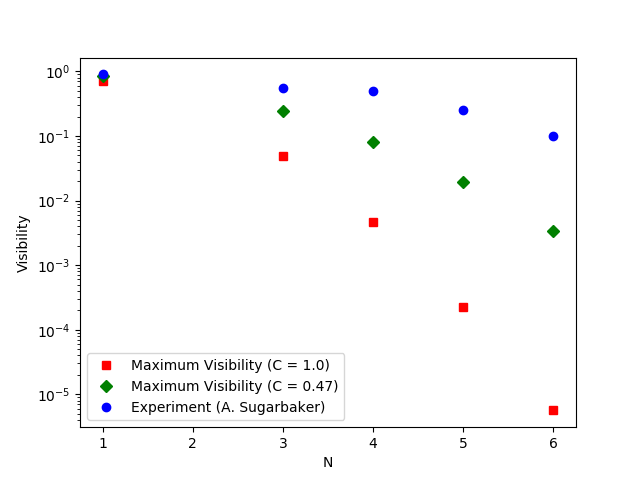
\includegraphics[width=.49\textwidth]{MinDR_1.png} 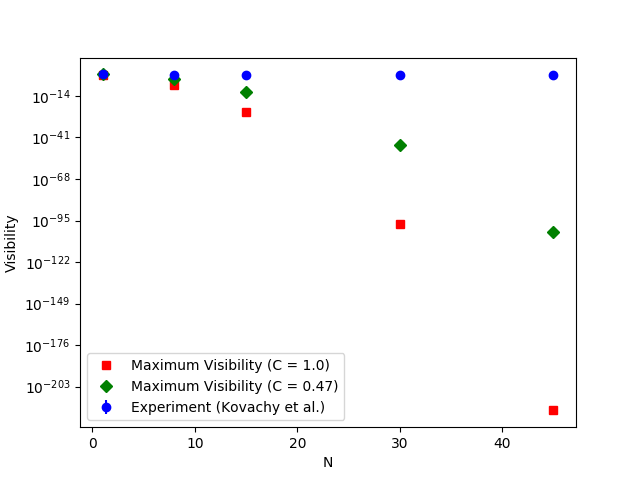
\includegraphics[width=.49\textwidth]{MinDR_2.png}\qquad\qquad
\caption{Comparing the maximum visibility estimate derived using decoherence rate minimization to values measured in atomic fountain interference experiments. Here $M_\oplus  = 6 \times 10^{24}$ kg, $R_\oplus 6\times 10^3$ km, $\frac{\hbar k}{m_a} = 5.8 $ mm/s, $m_a = 1.4\times10^{-25}$ kg, $T = 1.15$ s for ref.~\cite{sugarbaker} (left), and $T = 1.04$ s for ref.~\cite{kovachy} (right).}
\label{vis_DR}
\end{figure*}

As seen in fig~\ref{vis_DR}, $V_{deco}$ is much less than the visibilities determined experimentally by Kovachy et al. and Sugarbaker in ref.~\cite{kovachy, sugarbaker}. Though treating the earth as a composite body increases the maximum visibilities predicted by the model, the values are still many orders of magnitude too small. Considering the earth as a point particle ($C=1$), the predicted maximum visibilities are less than the measured values by factors up to $\sim 10^{200}$. Even for the composite body correction ($C=0.47$), the predicted values are less than the measured values by factors up to $\sim 10^{100}$ . However, the maximum visibility estimate must be derived using heating rate minimization as well in order to determine which estimate is the true theoretical maximum. 

%%%%%%%%%%%%%%%%%%%%%%%%%%%%%%%%%%%%%%%%%%%%%%%%%%%%%%

\section{Maximum Visibility Through Heating Rate Minimization}

To derive the maximum visibility estimate through heating rate minimization, I first rewrite the master equation for a two-particle system without assuming that the measurement strength of interactions involving the atom are equal to the measurement strength of interactions involving the earth. This assumption can not be made here as it was for the decoherence rate minimization method because it is not yet known if the maximum visibility estimate in this case is unchanged under this assumption.

\beq
 \dot{\rho} = -\frac{i}{\hbar}[\h H_0+ \h V_0, \rho] 
 -\bigg(\frac{1}{4D_a}+\frac{K^2D_\oplus}{4\hbar^2}\bigg)[\h x_a, [\h x_a,\rho]]
  -\bigg(\frac{1}{4D_\oplus}+\frac{K^2D_a}{4\hbar^2}\bigg)[\h x_\oplus, [\h x_\oplus,\rho]]
 \label{MasterEqn_HeatingRatePreMin}
 \eeq

In eq.~\eqref{MasterEqn_HeatingRatePreMin}, one particle is again set to be a $^{87}$Rb atom and the other is set to be the earth. In this equation's middle term, it can be seen that the atom first undergoes a measurement interaction with one ancilla with strength $D_a$, then the atom undergoes a feedback interaction with the other ancilla that depends on both $K$ and the measurement strength of the earlier ancilla-earth interaction, $D_\oplus$. The reverse is true for final term which describes the interactions between the ancillae and the earth.
 
Heating rate, $R_h$, is defined as the average rate of change of the system's kinetic energy with respect to time due to energy being introduced into the system. The kinetic energy of the system is described by $\h H_0 = \frac{\h p_a^2}{2m_a} + \frac{\h p_\oplus^2}{2m_\oplus}$. Therefore the heating rate can be written as

\begin{eqnarray}
R_h &=& \left\langle \frac{d}{dt} \h H_0 \right\rangle \nonumber \\
&=& \frac{d}{dt} \text{Tr} \left\lbrack  \h H_0 \rho \right\rbrack \nonumber \\
&=& \text{Tr} \left\lbrack \h H_0 \dot \rho \right\rbrack \,. \label{defhrate}
\label{MasterEqn_HeatingRatePreMin}
\end{eqnarray}

where $\dot \rho$ is given by eq.~\eqref{MasterEqn_HeatingRatePreMin}. From this, it can be shown that $R_h$ can be written as

\beq
 R_h = \frac{\hbar^2}{m_a}\bigg(\frac{1}{4D_a}+\frac{K^2D_\oplus}{4\hbar^2}\bigg)
  + \frac{\hbar^2}{m_\oplus}\bigg(\frac{1}{4D_\oplus}+\frac{K^2D_a}{4\hbar^2}\bigg).
 \label{HeatingRate}
 \eeq
 
The minimum of heating rate occurs where $\frac{\partial R_h}{\partial D_a} = \frac{\partial R_h}{\partial D_\oplus} = 0$, corresponding to
 
 \beq
 D_a = \frac{\hbar}{K} \sqrt{\frac{M_\oplus}{m_a}}\,,\,\,\,\,\,\,\,\,\,\,\,\,\,\,\,\,\,\,D_\oplus = \frac{\hbar}{K} \sqrt{\frac{m_a}{M_\oplus}}.
 \label{Datom}
% \label{Dearth}
 \eeq
 
Substituting eq.~\eqref{Datom} into eq.~\eqref{HeatingRate} yields the master equation assuming the heating rate is the minimum heating rate.
 
 \beq
 \dot{\rho} = -\frac{i}{\hbar}[\h H_0+\h V_0, \rho] 
 -\frac{K}{2\hbar}\bigg(\sqrt{\frac{m_a}{M_\oplus}}[\h x_a, [\h x_a,\rho]]
 + \sqrt{\frac{M_\oplus}{m_a}}[\h x_\oplus, [\h x_\oplus,\rho]]\bigg).
 \label{MasterEqn_HeatingRatePostMin}
 \eeq
 
Using the definition of the atom's decoherence rate stated previously, the decoherence rate under the minimum heating rate constraint is given by

\beq
\label{gamma_minHR}
\Gktm=\frac{K}{2\hbar}\sqrt{\frac{m_a}{M_\oplus}}\Delta x(t)^2.
\eeq

Using $K = 2\frac{Gm_1m_2}{d^3}$ and eq.~\eqref{SP_size} to rewrite eq.~\eqref{gamma_minHR} in terms of experiment parameters gives

\beq
\label{gamma_minHR2}
\Gktm=\frac{4G\hbar M_\oplus N^2  k^2 t^2}{m_a R_\oplus^3}\sqrt{\frac{m_a}{M_\oplus}}.
\eeq

Finally, we obtain the maximum visibility estimate predicted by the KTM model through heating rate minimization using eq.~\eqref{vis_explicit},

 \beq
 V_{\text{heat}} =  e^{-\frac{8 G \hbar k^2 M_\oplus T^3 N^2}{3 m_a R_\oplus^3}\sqrt{\frac{m_a}{M_\oplus}}}.
 \eeq

 \begin{figure*}[ht!]
 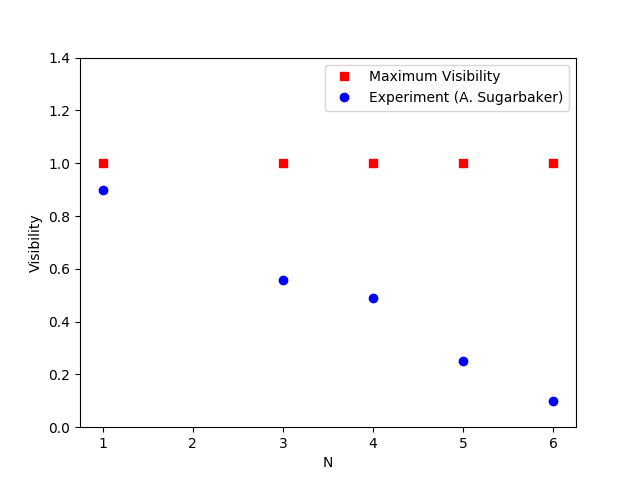
\includegraphics[width=.49\textwidth]{MinHR_1.png} 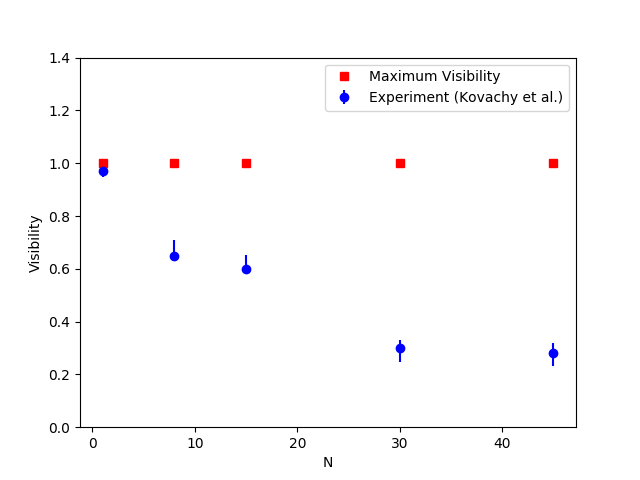
\includegraphics[width=.49\textwidth]{MinHR_2.png}\qquad\qquad
\caption{Comparing the maximum visibility estimate derived using heating rate minimization to values measured in atomic fountain interference experiments. Here $M_\oplus  = 6 \times 10^{24}$ kg, $R_\oplus 6\times 10^3$ km, $\frac{\hbar k}{m_a} = 5.8 $ mm/s, $m_a = 1.4\times10^{-25}$ kg, $T = 1.15$ s for ref.~\cite{sugarbaker} (left), and $T = 1.04$ s for ref.~\cite{kovachy} (right).}
\label{vis_HR}
\end{figure*}

Note, this maximum visibility estimate is very similar to the estimate from the decoherence minimization rate method when $C = 1$. They only differ by a factor of $\sqrt{\frac{m_a}{M_\oplus}}$ in the exponent.

 \beq
 V_{heat} = V_{deco}(C=1)^{\sqrt{\frac{m_a}{M_\oplus}}}
 \eeq

Since $M_\oplus$ is much greater than $m_a$, $\sqrt{\frac{m_a}{M_\oplus}}$ is much less than $1$. This means that $V_{heat}$ is larger than $V_{deco}$ for $N>0$, and $V_{heat}$ is therefore the true theoretical maximum visibility. $V_{heat}$ is greater than the visibilities experimentally determined by Kovachy et al. and Sugarbaker \cite{kovachy, sugarbaker}, as seen in fig~\ref{vis_HR}. Since the composite body correction only increase maximum visibility estimates, as seen in fig~\ref{vis_DR}, introducing the correction is not necessary using this method. When approximating the earth as a point particle, $V_{heat}$ is already at the maximum possible value of 1 visually on the scales shown in fig~\ref{vis_HR}. Note that the experimentally determined visibilities do not follow $V_{heat}$. $V_{heat}$ is a prediction of the atom's visibility assuming all decoherence is due to gravity, so the experiments' values being less then the theory's predictions suggests that the atoms in the atomic fountain experiments may be interacting with their environment through channels other than gravity.

%%%%%%%%%%%%%%%%%%%%%%%%%%%%%%%%%%%%%%%%%%%%%%%%%%%%%

\section{Testing for Classicality}

To confirm that this model is indeed a classical channel, there is a test that can be done outlined in ref.~\cite{KTM2}. First, the master equation under the constraint that produced the true theoretical maximum visibility, eq.~\eqref{MasterEqn_HeatingRatePostMin} in this case, must first be written in the form

\beq
 \dot{\rho} = -\frac{i}{\hbar}[\h H_0, \rho] 
 - ig[\h x_1 \h x_2, \rho]
 -\frac{1}{4}\sum_{k=1}^2Y_{ij}[\h x_i, [\h x_j,\rho]].
 \label{MasterEqn_EigenvalueGenForm}
 \eeq
 
If the matrix $Y-2ig\sigma$, where $\sigma = \begin{pmatrix} 
0 & 1 \\
-1 & 0 
\end{pmatrix}$, has no negative eigenvalues, then the model never increases entanglement and is therefore a classical channel. Using $\h V_0 = K\h x_1\h x_2$, eq.~\eqref{MasterEqn_HeatingRatePostMin} can be written as

\beq
 \dot{\rho} = -\frac{i}{\hbar}[\h H_0, \rho] 
 - i\frac{K}{\hbar}[\h x_1 \h x_2, \rho]
 -\frac{K}{2\hbar}\bigg(\sqrt{\frac{m_a}{M_\oplus}}[\h x_a, [\h x_a,\rho]]
 + \sqrt{\frac{M_\oplus}{m_a}}[\h x_\oplus, [\h x_\oplus,\rho]]\bigg).
 \label{MasterEqn_EigenvalueGenForm}
 \eeq

With the master equation in this form, $Y-2ig\sigma$ can easily be determined.

\beq
g = \frac{K}{\hbar}
\eeq

\beq
Y = \frac{2K}{\hbar}\begin{pmatrix} 
\sqrt{\frac{m_a}{M_\oplus}} & 0 \\
0 & \sqrt{\frac{M_\oplus}{m_a}}
\end{pmatrix}
\eeq

\beq
Y-2ig\sigma =  \frac{2K}{\hbar}\begin{pmatrix} 
\sqrt{\frac{m_a}{M_\oplus}} & -i \\
i & \sqrt{\frac{M_\oplus}{m_a}}
\end{pmatrix}
\eeq

The eigenvalues of $Y-2ig\sigma$ are 0 and $\frac{2K(m_1 + m_2)}{\hbar \sqrt{m_1m_2}}$, both of which are non-negative, therefore pairwise gravity is in fact a classical channel.

%%%%%%%%%%%%%%%%%%%%%%%%%%%%%%%%%%%%%%%%%%%%%%%%%%%%%%

\section{Conclusion}
Maximum visibility estimates from modelling gravity as pairwise classical channel have been made, and these estimates were be compared to visibility measurements made in atomic fountain interference experiments \cite{kovachy, sugarbaker}. Altamirano et al. derived a maximum visibility estimate through minimizing the atom's decoherence rate, however, this estimate predicts far greater gravitational decoherence than experiments have determined. When approximating the earth as a point particle, the maximum visibility estimate predicts values of factors up to $\sim 10^{200}$ less than experiment. Even when approximating the earth as a composite sphere, the maximum visibility estimate predicts values of factors up to $\sim 10^{100}$ less than experiment \cite{P3}.

However, it has been shown that the maximum visibility estimate determined using heating rate minimization is the true theoretical maximum visibility. The true theoretical maximum visibility is greater than the results from the atomic fountain experiments. This suggests that gravity may be a pairwise classical channel, it is yet to be experimentally disproven. The experimental values being less than the theoretical maximum suggests that the atoms in the experiments interact with their environment and decohere through channels other than just gravity. It is doubtful that atomic fountain experiments with reduced noise would be effective to better test the validity of this model. The predicted gravitational decoherence is so minute, that the noise present in the experiment would have to be unattainably close to zero for gravity to be the dominant source of decoherence. Determining new methods to measure gravitational decoherence is an interesting topic for further discussion.

The next logical step to take regarding this research is to determine if gravity could be a global local classical channel. The global case has to yet been investigated in depth. This research would involve deriving the master equation for the global case, then comparing maximum visibility estimates through both decoherence rate minimization and heating rate minimization to the results from the atomic fountain experiments.

%%%%%%%%%%%%%%%%%%%%%%%%%%%%%%%%%%%%%%%%%%%%%%%%%%%%%%

\section{Acknowledgments}
I would like to thank my supervisor, Professor Robert Mann, and Natacha Altamirano for the guidance and direction they offered throughout the course of this project. Completing so much within the time constraints of the project would have been impossible without their assistance.

%%%%%%%%%%%%%%%%%%%%%%%%%%%%%%%%%%%%%%%%%%%%%%%%%%%%%%
\begingroup\raggedright\begin{thebibliography}{10}

%\section{References}

\bibitem{PI}
Quantum Gravity. (n.d.). Retrieved from https://www.perimeterinstitute.ca/research/research-areas/quantum-gravity.

\bibitem{no_QG_evidence}
D.~N. Page and C.~D. Geilker, ``{Indirect Evidence for Quantum Gravity},''
\href{http://dx.doi.org/10.1103/PhysRevLett.47.979}{{\em Phys. Rev. Lett.}
  {\bfseries 47}, 979--982 (1981)}.
%%CITATION = PRLTA,47,979;%%.

\bibitem{KTM1}
D.~{Kafri} and J.~M. {Taylor}, ``{A noise inequality for classical forces},''
  {\em ArXiv e-prints} (2013), \href{http://arxiv.org/abs/1311.4558}{{\ttfamily
  arXiv:1311.4558 [quant-ph]}}.

\bibitem{KTM2}
D.~Kafri, J.~M. Taylor, and G.~J. Milburn, ``{A classical channel model for
  gravitational decoherence},''
  \href{http://dx.doi.org/10.1088/1367-2630/16/6/065020}{{\em New J. Phys.}
  {\bfseries 16}, 065020 (2014)},
\href{http://arxiv.org/abs/1401.0946}{{\ttfamily arXiv:1401.0946 [quant-ph]}}.
%%CITATION = ARXIV:1401.0946;%%.

\bibitem{KTM3}
D.~Kafri, G.~J. Milburn, and J.~M. Taylor, ``{Bounds on quantum communication
  via Newtonian gravity},''
\href{http://dx.doi.org/10.1088/1367-2630/17/1/015006}{{\em New J. Phys.}
  {\bfseries 17}, 015006 (2015)}.
%%CITATION = NJOPF,17,015006;%%.

\bibitem{P6}
N.~Altamirano, P.~Corona-Ugalde, K.~E. Khosla, R.~B. Mann, and M.~Zych, ``{Emergent dark energy via decoherence in quantum
interactions},''{(2017)}
   \href{https://arxiv.org/pdf/1605.05980.pdf},
{{\ttfamily arXiv:1605.05980v2 [gr-qc]}}.
%%CITATION = ARXIV:1605.04312;%%.

\bibitem{P2}
N.~Altamirano, P.~Corona-Ugalde, R.~B. Mann, and M.~Zych, ``{Unitarity,
  Feedback, Interactions -- Dynamics Emergent from Repeated Measurements},''
   \href{http://iopscience.iop.org/article/10.1088/1367-2630/aa551b}{{\em New Journal of Physics}
 (2016)},
\href{http://arxiv.org/abs/1605.04312}{{\ttfamily arXiv:1605.04312
  [quant-ph]}}.
%%CITATION = ARXIV:1605.04312;%%.

\bibitem{P3}
N.~Altamirano, P.~Corona-Ugalde, R.~B. Mann, and M.~Zych, ``{Gravity is not a Pairwise Classical Channel},''
   {(2016)},
\href{http://arxiv.org/abs/1612.07735v1}{{\ttfamily arXiv:1612.07735v1
  [quant-ph]}}.
%%CITATION = ARXIV:1605.04312;%%.

\bibitem{kovachy}
T.~Kovachy, P.~Asenbaum, C.~Overstreet, C.~Donnelly, S.~Dickerson,
  A.~Sugarbaker, J.~Hogan, and M.~Kasevich, ``Quantum superposition at the
  half-metre scale,'' {\em Nature} {\bfseries 528}, 530--533 (2015).

\bibitem{sugarbaker}
A.~{Sugarbaker}, ``{ Atom interferometry in a 10 m fountain, Stanford, 2014},''
  {\em Ph.D. thesis} (2014).

\end{thebibliography}\endgroup

\end{document}






















